%*************************************
% บทที่ 3
%*************************************
\chapterTitle{3}{วิธีการดำเนินงาน}

\hspace*{1.5em} %ย่อหน้า
ในการจัดทำปริญญานิพนธ์ฉบับนี้ ผู้จัดทำได้เลือกใช้ LaTeX เป็นเครื่องมือหลักในการจัดรูปแบบเอกสารทั้งหมด ซึ่งช่วยให้การสร้างเอกสารทางวิชาการที่มีโครงสร้างซับซ้อนเป็นไปได้อย่างมีประสิทธิภาพและเป็นมาตรฐาน โดยอ้างอิงตามไฟล์คลาส \textbf{project\_report.cls} ที่กำหนดไว้ รายละเอียดของวิธีการดำเนินงาน มีดังต่อไปนี้

\section{การเตรียมสภาพแวดล้อมการทำงาน}

\hspace*{1.5em} %ย่อหน้า
ก่อนเริ่มต้นการเขียน ผู้จัดทำได้ดำเนินการเตรียมความพร้อมของสภาพแวดล้อมที่จำเป็นสำหรับการใช้งาน LaTeX ดังนี้

\begin{mycustomenum2}
    \item \textbf{การติดตั้ง TeX Distribution} ผู้จัดทำได้ติดตั้ง MiKTeX ซึ่งเป็น TeX Distribution ที่มีความยืดหยุ่นในการติดตั้งแพ็กเกจแบบ On-the-fly (ติดตั้งเมื่อใช้งาน) และครอบคลุมคอมไพเลอร์ LaTeX แพ็กเกจที่จำเป็น รวมถึงเครื่องมือพื้นฐานสำหรับการจัดทำเอกสาร โดยเฉพาะอย่างยิ่ง XeLaTeX ซึ่งเป็นคอมไพเลอร์หลักที่รองรับการใช้งานฟอนต์ระบบและภาษาไทยได้อย่างสมบูรณ์
    \item \textbf{โปรแกรมแก้ไขข้อความ (Text Editor) / IDE} เพื่อเพิ่มประสิทธิภาพในการเขียนและแก้ไขโค้ด LaTeX ผู้จัดทำได้ใช้เครื่องมือดังต่อไปนี้
    \begin{mycustomenum2}
        \item \textbf{TeXworks} เป็นโปรแกรมแก้ไขข้อความและสภาพแวดล้อมการทำงานแบบครบวงจร (IDE) ที่มาพร้อมกับการติดตั้ง MiKTeX ซึ่งมีฟังก์ชันการไฮไลต์โค้ด การตรวจสอบไวยากรณ์ การคอมไพล์เอกสารด้วย XeLaTeX และการแสดงผลลัพธ์เป็น PDF ได้อย่างรวดเร็ว
        \item \textbf{Overleaf} เป็นแพลตฟอร์มออนไลน์สำหรับการเขียน LaTeX ร่วมกัน (Collaborative LaTeX Editor) ที่ช่วยให้ผู้จัดทำสามารถทำงานได้จากทุกที่โดยไม่จำเป็นต้องติดตั้งซอฟต์แวร์บนเครื่อง และสามารถทำงานร่วมกับผู้อื่นได้แบบเรียลไทม์ พร้อมการคอมไพล์เอกสารและแสดงผลลัพธ์แบบทันที
    \end{mycustomenum2}
\end{mycustomenum2}


\section{โครงสร้างเอกสาร LaTeX และการตั้งค่าพื้นฐาน}

\hspace*{1.5em} %ย่อหน้า
เอกสารปริญญานิพนธ์ฉบับนี้ถูกจัดโครงสร้างโดยใช้ไฟล์คลาส \textbf{project\_report.cls} ซึ่งกำหนดรูปแบบพื้นฐานและแพ็กเกจที่จำเป็นไว้ล่วงหน้า ทำให้การจัดรูปแบบเอกสารเป็นไปตามข้อกำหนด ดังรายละเอียดต่อไปนี้

\subsection{คลาสเอกสารและขนาดกระดาษ}

\hspace*{1.5em} %ย่อหน้า
รูปเล่มโครงงานที่สร้างขึ้นฉบับนี้ใช้ \textbf{\textbackslash documentclass[12pt,a4paper,oneside]\{book\}} ตามที่กำหนดไว้ใน \textbf{project\_report.cls} เพื่อให้ได้โครงสร้างแบบหนังสือขนาด A4 แบบหน้าเดียว และใช้ \textbf{\textbackslash RequirePackage[a4paper,top=1.5in,bottom=1in,left=1.5in,right=1in]\{geometry\}} เพื่อกำหนดระยะขอบกระดาษตามมาตรฐาน


\subsection{การตั้งค่าฟอนต์และภาษา}
\begin{mycustomitem2}
    \item \textbf{ฟอนต์ภาษาไทย} ไฟล์คลาสได้กำหนดให้ใช้ \textbf{THSarabunNew} เป็นฟอนต์หลักของเอกสาร (\textbf{\textbackslash setmainfont[Path=font/,...]\{THSarabunNew\}}) ซึ่งผู้จัดทำได้ตรวจสอบว่ามีไฟล์ฟอนต์ดังกล่าวอยู่ในโฟลเดอร์ \textbf{font/} ที่เหมาะสม และใช้ \textbf{\textbackslash XeTeXlinebreaklocale th} เพื่อรองรับการตัดคำภาษาไทยอย่างถูกต้อง
    \item \textbf{ขนาดฟอนต์เริ่มต้น} ค่าเริ่มต้นให้ใช้ฟอนต์ขนาด 16pt (\textbf{\textbackslash fontsize\{16\}\{16\}\textbackslash selectfont}) สำหรับเนื้อหาหลัก
\end{mycustomitem2}


\subsection{การจัดการย่อหน้า}
\hspace*{1.5em} %ย่อหน้า
การจัดย่อหน้าได้มีการใช้ \textbf{\textbackslash hspace*{1.5em}} โดยตัวอย่างการใช้งานสามารถดูได้ดังภาพที่ \ref{fig3:ExampleHspace}

\begin{figure}[htbp]
\centering
\adjustbox{frame, width=1.0\textwidth}{%สร้างกรอบของภาพ
    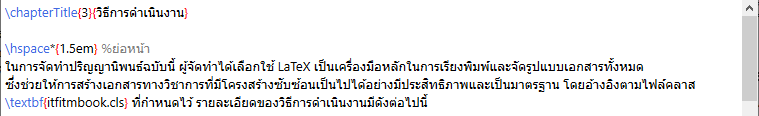
\includegraphics[width=1.0\textwidth]{Image/ExampleHspace.png}
}
\caption{\fontSixTeen{ตัวอย่างการเขียนคำสั่งสำหรับการย่อหน้าในเอกสาร}}
\label{fig3:ExampleHspace}
\end{figure}

\hspace*{1.5em} %ย่อหน้า
จากภาพที่ \ref{fig3:ExampleHspace} ในส่วนของตัวเลข 1.5 ที่ระบุไว้ในคำสั่ง hspace ผู้ใช้สามารถปรับได้เอง เมื่อต้องการย่อหน้ามากขึ้นหรือน้อยลงตามต้องการ

\subsection{แพ็กเกจที่จำเป็น}

\begin{mycustomitem2}
    \item \textbf{graphicx} ใช้สำหรับการแทรกรูปภาพด้วยคำสั่ง \textbf{\textbackslash includegraphics\{\}}
    \item \textbf{setspace} ใช้สำหรับการปรับระยะห่างระหว่างบรรทัด (แม้ว่าใน \textbf{.cls} ไฟล์จะ commented out \textbf{\textbackslash setstretch\{1.1\}} แต่สามารถเปิดใช้ใน \textbf{.tex} ได้)
    \item \textbf{titlesec} และ \textbf{tocloft} สำหรับการปรับแต่งรูปแบบหัวข้อและสารบัญ ตลอดจนสารบัญภาพและสารบัญตาราง
    \item \textbf{fancyhdr} และ \textbf{emptypage} สำหรับการกำหนดรูปแบบหัวกระดาษและท้ายกระดาษ รวมถึงการจัดการเลขหน้า
    \item \textbf{tcolorbox} สำหรับการสร้างกรอบข้อความ (code/box)
    \item \textbf{booktabs}, \textbf{float}, \textbf{tabularx}, \textbf{ragged2e}, \textbf{caption} สำหรับการสร้างและจัดรูปแบบตารางอย่างมืออาชีพ รวมถึงการกำหนดคำบรรยายใต้ภาพและตารางให้มีฟอนต์และขนาดตามที่กำหนด (\textbf{\textbackslash captionsetup[figure]}, \textbf{\textbackslash captionsetup[table]})
    \item \textbf{glossaries} สำหรับการสร้างอภิธานศัพท์และคำย่อ
    \item \textbf{hyperref} สำหรับการสร้างลิงก์ภายในเอกสารและลิงก์ภายนอกเอกสารพร้อมการกำหนดสีลิงก์
    \item \textbf{enumitem} สำหรับการปรับแต่งรายการแบบลำดับ (enumerate) และแบบจุด (itemize) โดยมีการกำหนดรูปแบบ \textbf{mycustomenum2}, \textbf{mycustomenum}, \textbf{mycustomitem} สำหรับรายการหลายระดับ
\end{mycustomitem2}

\subsection{การจัดโครงสร้างไฟล์}
\hspace*{1.5em} %ย่อหน้า
เพื่อให้การจัดการเอกสารขนาดใหญ่เป็นระบบ บทแต่ละบทได้ถูกแบ่งแยกส่วนสำคัญของปริญญานิพนธ์ออกเป็นไฟล์ย่อย ๆ เช่น \textbf{Main.tex} (เป็นไฟล์หลักที่รวมทุกส่วนของเล่มเข้าด้วยกัน), \textbf{Chapter1.tex}, \textbf{Chapter2.tex}, \textbf{Bibliography.bib} เป็นต้น และใช้คำสั่ง \textbf{\textbackslash include\{filename\}} ในไฟล์ \textbf{Main.tex} หลัก เพื่อประกอบรวมเป็นเอกสารฉบับสมบูรณ์


\section{การดำเนินการเขียนและการจัดรูปแบบ}
\hspace*{1.5em} %ย่อหน้า
ในการจัดรูปแบบเอกสารคำสั่งหลัก ๆ ได้กำหนดไว้ใน \textbf{project\_report.cls} ดังนี้

\subsection{การกำหนดบท (Chapter)}
\hspace*{1.5em} %ย่อหน้า
การกำหนดบทจะใช้คำสั่ง \textbf{\textbackslash chapterTitle\{<Chapter Number>\}\{<Chapter Title>\}} เช่น \textbf{\textbackslash chapterTitle\{3\}\{วิธีการดำเนินงาน\}} ซึ่งคำสั่งนี้จะจัดการการขึ้นหน้าใหม่ การใส่หัวข้อ "บทที่ X" และ "ชื่อบท" โดยอัตโนมัติ และรีเซ็ตเลขรูปภาพ/ตาราง/ส่วนย่อยให้เริ่มใหม่ในแต่ละบท

\subsection{การกำหนดหัวข้อรอง}
\hspace*{1.5em} %ย่อหน้า
การกำหนดหัวข้อรองจะใช้ \textbf{\textbackslash section\{...\}}, \textbf{\textbackslash subsection\{...\}} สำหรับหัวข้อและหัวข้อย่อย ซึ่งไฟล์คลาสได้กำหนดรูปแบบและระยะเยื้องของหัวข้อเหล่านี้ไว้แล้ว

\subsection{การใช้งานรูปภาพ}
\hspace*{1.5em} %ย่อหน้า
รูปภาพ (Figures) ถูกแทรกในเอกสารเพื่อแสดงแผนภาพ แผนผัง กราฟ หรือภาพหน้าจอของระบบ โดยใช้สภาพแวดล้อม \textbf{figure} พร้อมคำสั่ง \textbf{\textbackslash includegraphics} และ \textbf{\textbackslash caption} การจัดรูปแบบของคำบรรยายภาพเป็น \textbf{ฟอนต์หนาขนาด 16pt และจัดกึ่งกลาง} ซึ่งถูกกำหนดไว้ใน \textbf{\textbackslash captionsetup[figure]} ของ \textbf{project\_report.cls} โดยที่ไฟล์ภาพทั้งหมดได้ถูกจัดเก็บไว้ในโฟลเดอร์ย่อย \textbf{Image/} เพื่อความเป็นระเบียบและง่ายต่อการจัดการ ในส่วนของการกำหนดป้ายกำกับ (label) สำหรับรูปภาพ โดยกำหนดไว้ด้วยคำสั่ง \textbf{\textbackslash label\{fig3:ExampleTeXworksPhoto\}} ซึ่งสามารถอ้างอิงถึงรูปภาพนี้ในเนื้อหาเอกสารด้วยคำสั่ง \textbf{\textbackslash ref\{fig3:ExampleTeXworksPhoto\}} โดย LaTeX จะแปลงเป็นหมายเลขรูปภาพที่ถูกต้องโดยอัตโนมัติ

\begin{figure}[htbp]
\centering
\adjustbox{frame, width=1.0\textwidth}{%สร้างกรอบของภาพ
    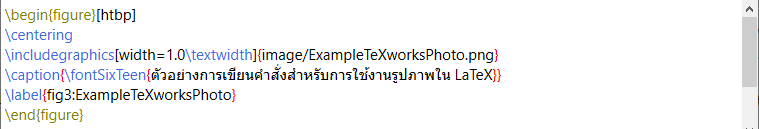
\includegraphics[width=1.0\textwidth]{Image/ExampleTeXworksPhoto.png}
}
\caption{\fontSixTeen{ตัวอย่างการเขียนคำสั่งสำหรับการใช้งานรูปภาพใน LaTeX}}
\label{fig3:ExampleTeXworksPhoto}
\end{figure}

\hspace*{1.5em} %ย่อหน้า
จากภาพที่ \ref{fig3:ExampleTeXworksPhoto} ในการปรับขนาดของรูปภาพให้เหมาะสมกับเอกสาร สามารถใช้ตัวเลือก \textbf{width} ในคำสั่ง \textbf{\textbackslash includegraphics} ซึ่งช่วยให้สามารถกำหนดความกว้างของรูปภาพสัมพันธ์กับความกว้างของหน้ากระดาษได้ ตัวอย่างเช่น \textbf{width=1.0\textbackslash textwidth} หมายถึง การกำหนดให้รูปภาพมีความกว้างเท่ากับความกว้างของเนื้อหาข้อความทั้งหมดบนหน้ากระดาษ (\textbf{\textbackslash textwidth}) ทำให้รูปภาพไม่ล้นขอบหรือเล็กเกินไป ด้วยการปรับค่าตัวเลข (เช่น 0.8) เพื่อปรับความกว้างของรูปภาพตามความเหมาะสม

\subsection{การใช้งานตาราง}
\hspace*{1.5em} %ย่อหน้า
ตาราง (Tables) ถูกใช้เพื่อนำเสนอข้อมูลเชิงตัวเลข คุณสมบัติ หรือข้อมูลเปรียบเทียบในรูปแบบที่เป็นระเบียบ โดยใช้สภาพแวดล้อม \textbf{table} ร่วมกับ \textbf{tabularx} เพื่อให้ตารางสามารถปรับความกว้างของคอลัมน์ได้อัตโนมัติ คำบรรยายตารางจะถูกจัดรูปแบบเป็น \textbf{ฟอนต์หนาขนาด 16pt} ตามที่กำหนดใน \textbf{\textbackslash captionsetup[table]} ของ \textbf{project\_report.cls}


\newpage
\begin{table}[h!]
    \centering
    \caption{\fontSixTeen ตัวอย่างการสร้างตารางด้วย LaTeX}
    \label{tab3:ExampleCreateTable}
    \fontSixTeen 
    \begin{tabularx}{\textwidth}{| c | X | r |} 
    \hline
    \textbf{กึ่งกลาง} 	& \textbf{ชิดซ้าย} 					& \textbf{ชิดขวา} \\
    \hline
    ข้อมูลตรงกลาง      & ข้อมูลนี้จะถูกจัดชิดซ้ายของคอลัมน์			& 1,234.56 		 \\
    หัวข้อ            & รายละเอียดเพิ่มเติม                     & 25 มิถุนายน 2568 \\
    100            	& ข้อความอาจจะยาวกว่านี้เพื่อแสดงการจัดตำแหน่ง & จำนวนรวม 		 \\
    \hline
    \end{tabularx}
\end{table}

\hspace*{1.5em} %ย่อหน้า
จากตารางที่ \ref{tab3:ExampleCreateTable} สร้างจากคำสั่งดังภาพที่ \ref{fig3:ExampleCreateTable} 

\begin{figure}[h!]
\centering
\adjustbox{frame, width=1.0\textwidth}{%สร้างกรอบของภาพ
    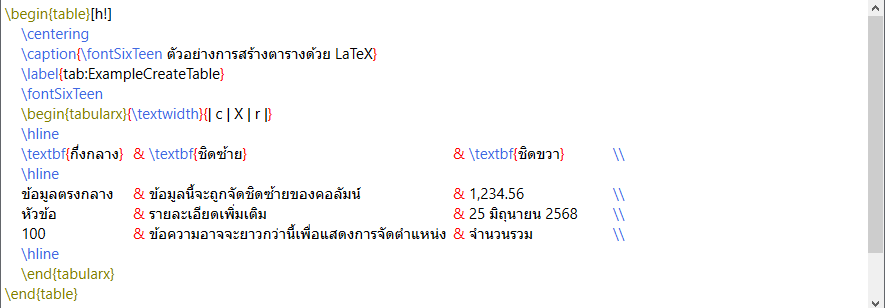
\includegraphics[width=1.0\textwidth]{Image/ExampleCreateTable.png}
}
\caption{\fontSixTeen{ตัวอย่างการเขียนคำสั่งสำหรับการสร้างตาราง}}
\label{fig3:ExampleCreateTable}
\end{figure}

\hspace*{1.5em} %ย่อหน้า
จากคำสั่งดังภาพที่ \ref{fig3:ExampleCreateTable} สามารถอธิบายเพิ่มเติมได้ดังนี้

\begin{mycustomitem}
    \item \textbf{\textbackslash begin\{tabularx\}\{\textbackslash textwidth\}\{...\}} ใช้เมื่อเริ่มต้นสภาพแวดล้อม \textbf{tabularx}
    \begin{mycustomitem}
        \item \textbf{\{\textbackslash textwidth\}} ใช้กำหนดให้ตารางมีความกว้างเต็ม \textbf{ความกว้างของข้อความ} (\textbf{\textbackslash textwidth}) ของหน้ากระดาษ
        \item \textbf{\{| c | X | r |\}} ส่วนนี้คือการ \textbf{กำหนดคุณสมบัติของแต่ละคอลัมน์}
        \begin{mycustomitem}
            \item \textbf{|} คือ การสร้าง \textbf{เส้นแนวตั้ง} คั่นระหว่างคอลัมน์
            \item \textbf{c} คือ คอลัมน์ที่เนื้อหา \textbf{จัดกึ่งกลาง} (centered)
            \item \textbf{X} คือ คอลัมน์พิเศษที่ \textbf{ปรับความกว้างอัตโนมัติ} (variable-width) เพื่อเติมเต็มพื้นที่ว่างที่เหลือ ทำให้ตารางมีความกว้างรวมตามที่กำหนด
            \item \textbf{r} คือ คอลัมน์ที่เนื้อหา \textbf{จัดชิดขวา} (right-aligned)
            \item \textbf{l} (เพิ่มเติม) คอลัมน์ที่เนื้อหา \textbf{จัดชิดซ้าย} (left-aligned)
        \end{mycustomitem}
    \end{mycustomitem}
    \item \textbf{\textbackslash hline} ใช้สำหรับสร้าง \textbf{เส้นแนวนอน} ในตาราง
    \item \textbf{\&} ใช้สำหรับ \textbf{คั่นระหว่างเซลล์} ในแต่ละแถว
    \item \textbf{\textbackslash\textbackslash} ใช้สำหรับ \textbf{ขึ้นบรรทัดใหม่} เพื่อเริ่มแถวใหม่ของตาราง
    \item \textbf{\textbackslash textbf\{\dots\}} ทำให้ข้อความ \textbf{ตัวหนา} เหมาะสำหรับหัวตาราง
\end{mycustomitem}

\newpage
\hspace*{1.5em} %ย่อหน้า
นอกเหนือจาก \textbf{h} ที่ใช้ในตัวอย่าง ยังมีตัวเลือกอื่น ๆ ที่สามารถใส่ใน \textbf{\textbackslash begin\{table\}[...]} เพื่อบอก LaTeX ว่าต้องการให้ตารางไปปรากฏที่ใด

\begin{mycustomitem}
    \item \textbf{h} (here) พยายามวางตาราง \textbf{ตรงตำแหน่งที่โค้ดปรากฏ} ในไฟล์
    \item \textbf{t} (top) พยายามวางตารางที่ \textbf{ด้านบนสุดของหน้า} ปัจจุบันหรือหน้าถัดไป
    \item \textbf{b} (bottom) พยายามวางตารางที่ \textbf{ด้านล่างสุดของหน้า} ปัจจุบันหรือหน้าถัดไป
    \item \textbf{p} (page) นำตารางไปรวมไว้ใน \textbf{หน้าเฉพาะที่รวบรวมตาราง/รูปภาพ} เท่านั้น
    \item \textbf{!} (override) ใช้ \textbf{ร่วมกับ} ตัวเลือกอื่นๆ (เช่น \textbf{[h!]}, \textbf{[t!]}) เพื่อ \textbf{บังคับ} ให้ LaTeX พยายามวางตามตำแหน่งที่ระบุให้ได้ แม้จะต้องละเมิดกฎการจัดวางบางอย่าง
\end{mycustomitem}

\hspace*{1.5em} %ย่อหน้า
นอกจากนี้ยังสามารถรวมตัวเลือกเหล่านี้ได้ เช่น \textbf{[htb!]} เพื่อให้ LaTeX พยายามวางจาก "here" ก่อน ถ้าไม่ได้ก็ "top" ถ้าไม่ได้ก็ "bottom" และใช้ \textbf{!} เพื่อบังคับ


\subsection{การสร้างรายการ (Lists)}
\hspace*{1.5em} %ย่อหน้า
สำหรับรายการแบบลำดับ ผู้จัดทำได้ใช้สภาพแวดล้อมที่กำหนดเองในไฟล์คลาส ได้แก่ \textbf{mycustomenum}, \textbf{mycustomenum2} (สำหรับรายการลำดับเลข) และ \textbf{mycustomitem} (สำหรับรายการด้วยเครื่องหมาย) ซึ่งมีการกำหนดระยะเยื้องและรูปแบบของตัวเลข/สัญลักษณ์นำหน้าด้วยเครื่องหมายขีด

\hspace*{1.5em} %ย่อหน้า
\textbf{ตัวอย่างการใช้ \textbf{mycustomenum}} 
\begin{mycustomenum}[label=1.1.\arabic*]
    \item รายการระดับที่ 1 รายการระดับที่ 1 รายการระดับที่ 1 รายการระดับที่ 1  รายการระดับที่ 1 รายการระดับที่ 1
    \item รายการระดับที่ 1
    \begin{mycustomenum}
        \item รายการระดับที่ 2
        \begin{mycustomenum}
            \item รายการระดับที่ 3
            \item รายการระดับที่ 3 รายการระดับที่ 3 รายการระดับที่ 3 รายการระดับที่ 3 
        \end{mycustomenum}
        \item รายการระดับที่ 2 รายการระดับที่ 2 รายการระดับที่ 2 รายการระดับที่ 2
    \end{mycustomenum}
    \item รายการระดับที่ 1
    \item รายการระดับที่ 1
\end{mycustomenum}

\newpage
\hspace*{1.5em} %ย่อหน้า
จากตัวอย่างการใช้งาน mycustomenum ข้างต้น ตัวอย่างคำสั่งแสดงได้ดังภาพที่ \ref{fig3:ExampleCreateEnum} 

\begin{figure}[htbp]
\centering
\adjustbox{frame, width=1.0\textwidth}{%สร้างกรอบของภาพ
    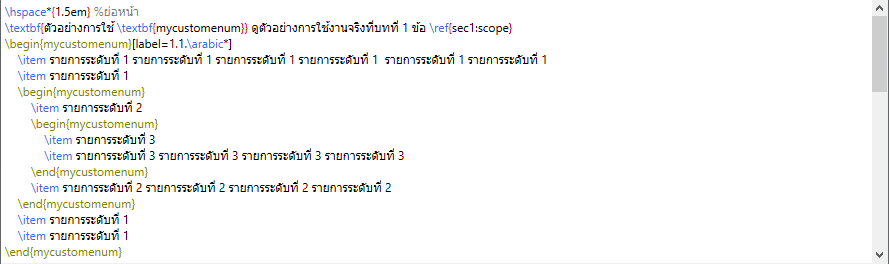
\includegraphics[width=1.0\textwidth]{Image/ExampleCreateEnum.png}
}
\caption{\fontSixTeen{ตัวอย่างการเขียนคำสั่งสำหรับการสร้างรายการด้วยคลาส mycustomenum}}
\label{fig3:ExampleCreateEnum}
\end{figure}



\hspace*{1.5em} %ย่อหน้า
\textbf{ตัวอย่างการใช้ \textbf{mycustomenum2}}
\begin{mycustomenum2}
    \item รายการระดับที่ 1
    \item รายการระดับที่ 1
    \begin{mycustomenum2}
        \item รายการระดับที่ 2
        \begin{mycustomenum2}
            \item รายการระดับที่ 3 รายการระดับที่ 3 รายการระดับที่ 3 รายการระดับที่ 3 รายการระดับที่ 3 รายการระดับที่ 3 รายการระดับที่ 3 
            \item รายการระดับที่ 3
        \end{mycustomenum2}
        \item รายการระดับที่ 2
        \item รายการระดับที่ 2
    \end{mycustomenum2}
\end{mycustomenum2}

\hspace*{1.5em} %ย่อหน้า
จากตัวอย่างการใช้งาน mycustomenum2 ข้างต้น ตัวอย่างคำสั่งแสดงได้ดังภาพที่ \ref{fig3:ExampleCreateEnum2} 

\begin{figure}[htbp]
\centering
\adjustbox{frame, width=1.0\textwidth}{%สร้างกรอบของภาพ
    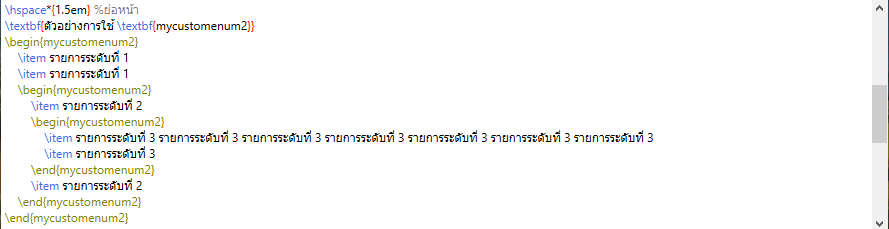
\includegraphics[width=1.0\textwidth]{Image/ExampleCreateEnum2.png}
}
\caption{\fontSixTeen{ตัวอย่างการเขียนคำสั่งสำหรับการสร้างรายการด้วยคลาส mycustomenum2}}
\label{fig3:ExampleCreateEnum2}
\end{figure}


\hspace*{1.5em} %ย่อหน้า
\textbf{ตัวอย่างการใช้ \textbf{mycustomitem}}
\begin{mycustomitem}
    \item รายการระดับที่ 1
    \item รายการระดับที่ 1
    \begin{mycustomitem}
        \item รายการระดับที่ 2
        \begin{mycustomitem}
            \item รายการระดับที่ 3 รายการระดับที่ 3 รายการระดับที่ 3 รายการระดับที่ 3 รายการระดับที่ 3 รายการระดับที่ 3 รายการระดับที่ 3 
            \item รายการระดับที่ 3
        \end{mycustomitem}
        \item รายการระดับที่ 2
    \end{mycustomitem}
\end{mycustomitem}


\hspace*{1.5em} %ย่อหน้า
จากตัวอย่างการใช้งาน mycustomitem ข้างต้น ตัวอย่างคำสั่งแสดงได้ดังภาพที่ \ref{fig3:ExampleCreateItem} 

\begin{figure}[htbp]
\centering
\adjustbox{frame, width=1.0\textwidth}{%สร้างกรอบของภาพ
    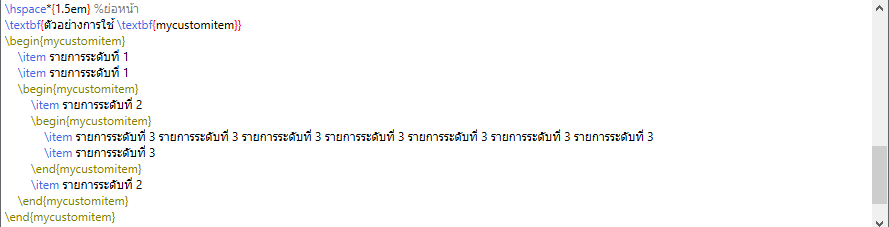
\includegraphics[width=1.0\textwidth]{Image/ExampleCreateItem.png}
}
\caption{\fontSixTeen{ตัวอย่างการเขียนคำสั่งสำหรับการสร้างรายการด้วยคลาส mycustomitem}}
\label{fig3:ExampleCreateItem}
\end{figure}


\hspace*{1.5em} %ย่อหน้า
\textbf{ตัวอย่างการใช้งาน mycustomenum2 และ mycustomitem ร่วมกัน}
\begin{mycustomenum2}
    \item รายการระดับที่ 1
    \item รายการระดับที่ 1
    \begin{mycustomenum2}
        \item รายการระดับที่ 2
        \begin{mycustomitem}[leftmargin=0.7cm,labelwidth=0.7cm]
            \item รายการระดับที่ 3
            \item รายการระดับที่ 3
        \end{mycustomitem}
        \item รายการระดับที่ 2
        \begin{mycustomitem}[leftmargin=0.7cm,labelwidth=0.7cm]
            \item รายการระดับที่ 3
            \begin{mycustomitem}
                \item รายการระดับที่ 4
                \item รายการระดับที่ 4
            \end{mycustomitem}
            \item รายการระดับที่ 3
        \end{mycustomitem}
        \item รายการระดับที่ 2
        \item รายการระดับที่ 2
    \end{mycustomenum2}
    \item รายการระดับที่ 1
    \begin{mycustomenum2}
        \item รายการระดับที่ 2
        \begin{mycustomenum2}
            \item รายการระดับที่ 3
            \begin{mycustomitem}[leftmargin=0.7cm,labelwidth=0.7cm]
                \item รายการระดับที่ 4
                \item รายการระดับที่ 4
            \end{mycustomitem}
            \item รายการระดับที่ 3
            \item รายการระดับที่ 3
        \end{mycustomenum2}
        \item รายการระดับที่ 2
    \end{mycustomenum2}
    \item รายการระดับที่ 1
    \item รายการระดับที่ 1
\end{mycustomenum2}


\hspace*{1.5em} %ย่อหน้า
จากตัวอย่างการใช้งาน mycustomenum2 และ mycustomitem ร่วมกันข้างต้น ตัวอย่างคำสั่งแสดงได้ดังภาพที่ \ref{fig3:ExampleCreateEnum2MixItem}

\begin{figure}[htbp]
\centering
\adjustbox{frame, width=1.0\textwidth}{%สร้างกรอบของภาพ
    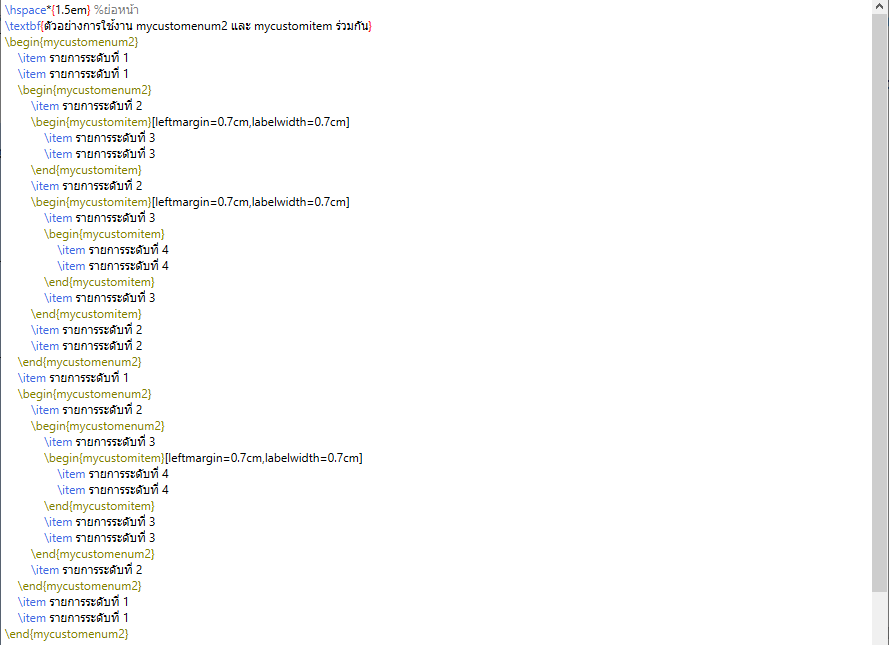
\includegraphics[width=1.0\textwidth]{Image/ExampleCreateEnum2MixItem.png}
}
\caption{\fontSixTeen{ตัวอย่างการเขียนคำสั่งสำหรับการสร้างรายการด้วยคลาส mycustomenum2 และ mycustomitem ร่วมกัน}}
\label{fig3:ExampleCreateEnum2MixItem}
\end{figure}



\subsection{การจัดการบรรณานุกรม}
\hspace*{1.5em} %ย่อหน้า
ในส่วนของการจัดการบรรณานุกรม มีรายละเอียดดังนี้

\begin{mycustomitem}
    \item ไฟล์ \textbf{.bib} (เช่น \textbf{Project\_999\_Bibliography.bib}) ได้ถูกสร้างไว้แล้วสำหรับรวบรวมข้อมูลบรรณานุกรมทั้งหมด
    \item ใช้คำสั่ง \textbf{\textbackslash addbibresource\{Project\_999\_Bibliography.bib\}} ใน Preamble ของเอกสาร และ \textbf{\textbackslash printbibliography} ในส่วนท้ายของเอกสารเพื่อสร้างหน้าบรรณานุกรม
    \item มีการกำหนดหัวเรื่องบรรณานุกรมด้วย \textbf{\textbackslash defbibheading\{mybibheading\}} ให้แสดง \textbf{บรรณานุกรม} และ \textbf{บรรณานุกรม (ต่อ)} พร้อมเลขหน้าตามที่กำหนดไว้ในไฟล์คลาส
\end{mycustomitem}


\hspace*{1.5em} %ย่อหน้า
ตัวอย่างการเขียนบรรณานุกรมในไฟล์ .bib แสดงได้ดังภาพที่ \ref{fig3:ExampleBib}

\begin{figure}[htbp]
\centering
\adjustbox{frame, width=1.0\textwidth}{%สร้างกรอบของภาพ
    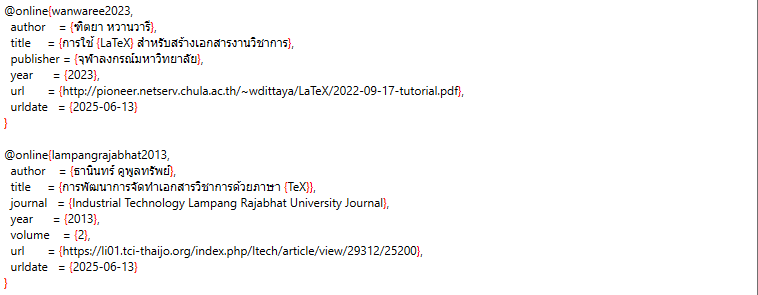
\includegraphics[width=1.0\textwidth]{Image/ExampleBib.png}
}
\caption{\fontSixTeen{ตัวอย่างการเขียนข้อมูลบรรณานุกรมใน bib file}}
\label{fig3:ExampleBib}
\end{figure}

\hspace*{1.5em} %ย่อหน้า
ตัวอย่างการเขียนอ้างอิงในเนื้อหา ด้วยคำสั่ง \textbf{\textbackslash parencite\{Tanya2008\}} แสดงได้ดังภาพที่ \ref{fig3:ExampleRefInContent}

\begin{figure}[htbp]
\centering
\adjustbox{frame, width=1.0\textwidth}{%สร้างกรอบของภาพ
    
\includegraphics[width=1.0\textwidth]{Image/ExampleRefInContent.png}
}
\caption{\fontSixTeen{ตัวอย่างการเขียนอ้างอิงในเนื้อหา}}
\label{fig3:ExampleRefInContent}
\end{figure}

